%% pwx321556's report latex template
%
%% report.tex
%
%% Copyright 2021 pwx321556

%*******************************************************************
%*
%*                           页面排版
%*
%*******************************************************************

\documentclass[12pt,a4paper,UTF8]{ctexart}
\usepackage{graphicx}                       %graphicx:插入图片
\usepackage{float}                          %float:图片浮动
\usepackage{subfigure}                      %subfigure:并排排版图片、竖向排版图片
\usepackage{caption}                        %caption:图像设置
\usepackage{booktabs}                       %booktabs:三线图,论文常用的表格风格
\usepackage{hyperref}                       %hyperref:超链接,和lastpage搭配
\usepackage{lastpage}                       %lastpage:获取总页数
\usepackage{setspace}                       %setspace:设置行间距等功能
\usepackage{geometry}                       %geometry:用于设置上下左右页边距
\usepackage{bibspacing}                     %bibspacing:自定义包,用于bib格式调整
\geometry{left=2.5cm,right=2.5cm,top=3.2cm,bottom=2.8cm}

% 页眉设置
\usepackage{fancyhdr}
	%fancyhdr:一个很强大的宏包,用于自定义设计页面风格并命名以供调用。
	\pagestyle{fancy}
	\rhead{实验十二 \;\; 保护模式操作系统}
	\lhead{操作系统原理 \ 实验报告}
	\cfoot{\thepage/\pageref{LastPage}}  %当前页\总页数
	%\rfoot{\today}                      %右下角显示日期
	%分别是右页眉、左页眉、中页脚、右页脚
    \renewcommand{\headrulewidth}{0.4pt} %页眉线
    %\renewcommand{\footrulewidth}{0.4pt}%页脚线
	%\renewcommand{\theenumi}{(\arabic{enumi})}%标号设置为(1)

%解决目录红框问题
\hypersetup{
    colorlinks=true,        %彩色显示超链接(否则出现框)
    linkcolor=black,        %文本链接颜色,默认为blue
    urlcolor=blue,          %URL颜色,默认为magenta
    %allcolors=black,
	pdfstartview=Fit,
	breaklinks=true
}

\title{\kaishu \LARGE 中山大学数据科学与计算机学院本科生实验报告\\
(2021学年春季学期)}
\date{}
\author{}

%------------------------------end----------------------------------


%*******************************************************************
%*
%*                           格式设置
%*
%*******************************************************************

\usepackage{color}
\usepackage[table,xcdraw]{xcolor}           %xcolor:提供表格等颜色
\usepackage{enumerate}                      %paralist,enumerate:自定义项目符号
\usepackage{paralist}
\usepackage{listings}                       %listings:用于排版各种代码;比如matlab的代码
\usepackage{array}                          %array:表格格式
\usepackage{multirow}                       %multirow, multicol:复杂表格
\usepackage{multicol}
\usepackage{bookmark}                       %bookmark:在PDF中生成索引标签

\definecolor{darkgreen}{RGB}{0, 100, 0}
%设置lstset环境(中间不可空行)
\lstset{
    aboveskip=3mm,                          %aboveskip:上边距
    belowskip=3mm,                          %belowskip:下边距
    xleftmargin=2em,                        %xleftmargin:左边距
    xrightmargin=2em,                       %xrightmargin:右边距
    frame=shadowbox,                        %frame:边框(tb:table, shadowbox:box)
    framerule=1pt,                          %framerule:边框线
    rulecolor=\color{gray!35},              %rulecolor:边框颜色
    backgroundcolor=\color{gray!5},         %backgroundcolor:背景颜色
    columns=flexible,                       %columns:字母间的空隙大小
    numbers=none,                           %numbers:代码行号(none/left/right)
    numberstyle=\tiny\color{gray},          %numberstyle:数字格式
    stepnumber=1,                           %stepnumber:每隔多少行记录一次行号
    basicstyle={\small\ttfamily},           %basicstyle:代码字体格式(\small, \footnotesize, \tt(等宽), \it(斜体), \bf等)
    keywordstyle=\color{blue},              %keywordstyle:代码关键词格式
    commentstyle=\color{darkgreen},         %commentstyle:注释格式
    stringstyle=\color{orange},             %stringstyle:字符串格式(mauve:淡紫色)
    showspaces=false,                       %showspaces:特别显示空格(加下划线)
    showstringspaces=false,                 %showstringspaces:显示字符串内空格(加下划线)
    breaklines=true,                        %breaklines:自动换行
    breakatwhitespace=false,                %breakatwhitespace:自动换行只在白空格生效
    tabsize=3,                              %tabsize:缩进大小
    morekeywords={}                         %morekeywords:自主设置关键词
}

%列表、枚举类型格式
\setlength{\leftmargin}{1.2em}              %左边界
\setlength{\parsep}{0ex}                    %段落间距
\setlength{\topsep}{1ex}                    %列表到上下文的垂直距离
\setlength{\itemsep}{0.3ex}                 %条目间距
\setlength{\labelsep}{0.3em}                %标号和列表项之间的距离,默认0.5em
\setlength{\itemindent}{1.1em}              %标签缩进量
\setlength{\listparindent}{0em}             %段落缩进量

\setlength{\pltopsep}{5pt}                  %修改表项行距
\let\itemize\compactitem
\let\enditemize\endcompactitem
\let\enumerate\compactenum
\let\endenumerate\endcompactenum
\let\description\compactdesc
\let\enddescription\endcompactdesc

%文献引用格式
\renewcommand\refname{参考资料}
\setlength{\bibspacing}{\baselineskip}      %参考资料行距为基础行距

%------------------------------end----------------------------------


%*******************************************************************
%*
%*                           字体设置
%*
%*******************************************************************

\usepackage{xeCJK}                          %xeCJK:中文字体(如楷体,作者和机构需要用到)的设置
\usepackage{amsmath}                        %amsmath:数学公式
\usepackage{amsfonts}                       %amsfonts:数学字体
\usepackage{amssymb}                        %amssymb:数学符号
\usepackage{fontspec}
\usepackage{fontsetup}

%中文字体设置:使用开源字体方正书宋,方正楷体和方正黑体
\setCJKmainfont[ItalicFont=FZKai-Z03S, BoldFont=FZHei-B01S]{FZShuSong-Z01S}
\renewcommand{\songti}{\CJKfontspec{Source Han Serif SC}}%用命令\songti调用思源宋体
\newcommand{\fzkaiti}{\CJKfontspec{方正楷体简体}}%用命令\fzkaiti调用方正楷体简体

\setlength{\parindent}{2em}                         %正文首行缩进两个汉字
\ctexset{section={format={\centering\bfseries\Large}}}
\ctexset{subsection={format={\bfseries\raggedright\large}}}
\ctexset{subsubsection={format=\bfseries\raggedright\normalsize}}
\newcommand{\tabincell}[2]{\begin{tabular}{@{}#1@{}}#2\end{tabular}}
\renewcommand{\contentsname}{\textbf{目录}}
\newcolumntype{P}[1]{>{\centering\arraybackslash}p{#1}} % P{4cm} = \centering p{4cm}


%------------------------------end----------------------------------


\begin{document}

% 封面设置
\begin{titlepage}
    \vspace*{-3cm}
\begin{figure}[h]
    \centering
    
\includegraphics[width=0.7\linewidth]{figs/sysu_logo.jpg}
\end{figure}
\begin{center}
    \Huge{\textbf{操作系统原理}}\\
    \Huge{\textbf{实验报告}}
\end{center}

\vspace*{3.5cm}
\begin{center}
        \large 
        实验名称\ \ \underline{\makebox[220pt]{实验十二\; 保护模式操作系统}} \\ 
        \vspace{0.3cm}
        \ \ \ 姓\; 名 \ \ \ \underline{\makebox[220pt]{潘文轩}} \\ 
        \vspace{0.3cm}
        \ \ \ 学\; 号 \ \ \ \underline{\makebox[220pt]{19335163}}\\
        \vspace{0.3cm}
        任教老师\ \ \underline{\makebox[220pt]{凌应标}}\\
        \vspace{0.3cm}
        \ \ \ 助\; 教 \ \ \ \underline{\makebox[220pt]{梁丰洲、车鑫恺}}\\
        \vspace{0.3cm}
        完成日期\ \ \underline{\makebox[220pt]{2021年 7 月 16 日}}\\
\end{center}
\end{titlepage}
\newpage

\section*{实验十二 \quad 保护模式操作系统}

\subsection*{一、实验目的}

\noindent 实验目的如下:

\renewcommand{\labelenumi}{(\theenumi)}
\begin{enumerate}
\item 学习保护模式操作系统的特点
\item 熟悉保护模式操作系统的实现方式
\item 对比实模式操作系统,理解保护模式的优点
\end{enumerate}

\noindent 实验内容如下:

\begin{enumerate}
\item 实现实模式到保护模式的跳转
\item 构造GDT、LDT,实现操作系统的分段内存管理
\item 通过调用门和远返回实现段间跳转和特权级转换
\item 构造页目录表与页表实现操作系统的分页内存管理
\item 实现中断与陷阱
\item 在已有的操作系统基础上引入FAT12文件系统组织方式
\item 利用Makefile文件汇编源代码、生产软盘映像文件
\end{enumerate}

\noindent 实验环境:Windows10/CentOS7 + DOSBOX + VirtualBox

\noindent 编译工具:NASM + GCC + LD

\subsection*{二、保护模式原理}

在IA32下,CPU有两种工作模式:实模式和保护模式。当我们打开自己的PC,开始时
CPU是工作在实模式下的,经过某种机制之后,才进入保护模式。在保护模式下,
CPU有着巨大的寻址能力,并为强大的32位操作系统提供了更好的硬件保障。

\subsubsection*{使用选择子访存}

保护模式下,访问的每一段内存,都需要提前跟CPU声明;描述一段内存无非需要它的:

\begin{enumerate}
\item 基地址
\item 长度
\item 扩展方式(向高地址还是向低地址)
\item 之后会用于维护访存秩序的特权级
\item 之后会与Cache有联系的“是否存在与主存”
\item 指明默认操作数大小。
\item 用途的粗分类
\end{enumerate}

正因为上述特征,才有了描述符那样奇怪而繁杂的标志位。而描述符(Descriptor)和选择子
(Selector)正是记录上述信息的载体。在保护模式中,一个程序的内存空间以段式内存方式管理,每个描述符描述了一个段的
主要信息。虽然段值仍然由原来16位的CS、DS
等寄存器表示,但此时它仅仅变成了一个索引,这个索引指向GDT(Global Descriptors Table)/
LDT(Local Descriptors Table)的一个表项,
表项中详细定义了段的起始地址、界限、属性等内容。
也就是说,由描述符组成的GDT的作用是用来提供段式存储机制,
这种机制是通过段寄存器和GDT中的描述符共同提供的。

\begin{figure}[htbp]
\centering
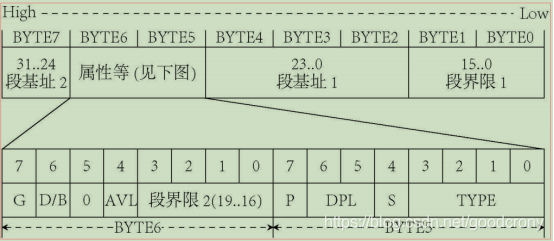
\includegraphics[width=0.7\textwidth]{figs/Descriptor.png}
\caption{段描述符组成}
\label{fig:Descriptor}
\end{figure}

介绍完描述符和GDT/LDT,再来介绍选择子。选择子是描述符在GDT/LDT中的偏移量,
也是程序访问描述符的索引。
选择子同样需要按表的方式组织,CPU中有一个专门的寄存器GDTR,指向段描述子表
GDT的首地址;段寄存器中则只需要记录用于检索该段的选择子在表中起始位置相对
GDT的偏移量,就足够描述一个段了。相应的,LDT也有对应的寄存器LDTR来存储
LDT的首地址。

x86中共有4个控制寄存器,cr0$\sim$3。涉及到保护模式开启的另一个标志位是
cr0的PE位。将该位设为1,便进入了保护模式。

\subsubsection*{任务寄存器TR}

TR用于寻址一个特殊的任务状态段(TaskState Segment,TSS)。TSS中包含着
当前执行任务的重要信息。

TR寄存器用于存放当前任务TSS段的16位段选择符、32位基地址、16位段长度和
描述符属性值。它引用GDT表中的一个TSS类型的描述符。指令LTR和STR分别用于
加载和保存TR寄存器的段选择符部分。当使用LTR指令把选择符加载进任务寄存器时,
TSS描述符中的段基地址、段限长度以及描述符属性会被自动加载到任务寄存器中。
当执行任务切换时,处理器会把新任务的TSS的段选择符和段描述符自动加载进
任务寄存器TR中。

\begin{figure}[htbp]
\centering
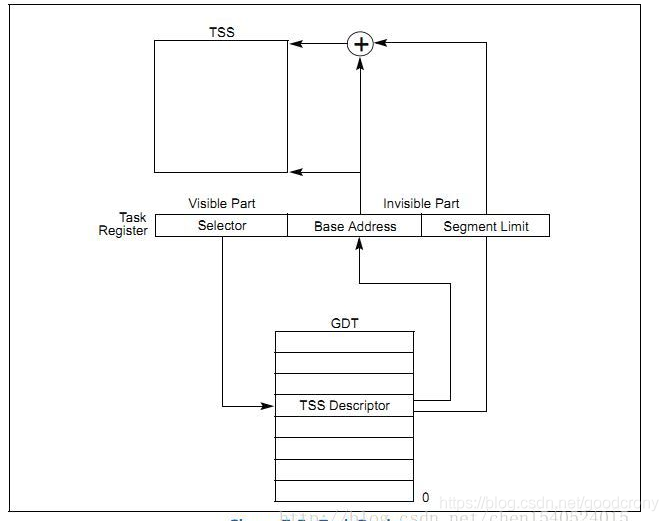
\includegraphics[width=0.7\textwidth]{figs/TSS.png}
\caption{TSS结构}
\label{fig:TSS}
\end{figure}

\subsubsection*{分页机制}

x86提供页式访存机制。通过“页目录--页表”两层的结构,将线性(逻辑)地址映射到物理地址。
一张页目录和一张页表和一张页都是4kb,4B/项*1024项。页目录中的每一项记录页表的物理首地址,页表每一项的都记录一张4kb页的物理首地址。
每个页目录/页表项的高20位表示物理地址的高12位(因为页都是按4kb分配的);低12位就用来记录和

\begin{itemize}
\item 高速缓存Cache
\item 页读写策略,
\item 是否全局页/页表
\end{itemize}

页目录需要通过cr3来指向其物理首地址,并把cr0中的PG位置位,来正式开启分页机制。

\subsubsection*{中断门}

门是x86中一类用来处理不同特权级代码之间进行控制转移的一种(保护的)格式。本质上它还是一个描述符,只是不同于代码段和数据段而已。
调用门,中断门,任务门,陷阱门他们都非常相似,他们都必须包含16位目标代码段的选择子,32位段内偏移量和特权级。
类似于GDT,每个中断例程都通过中断门来调用,这些256个中断门组成一个1KB的表(每项4B),由IDTR来指向中断向量表的首地址以及偏移量
之后每个对应中断发生时,都通过“中断向量---中断门---目标代码选择子”来实现调用中断例程。

\subsection*{三、代码分析}

\textbf{GDT段:}
GDT段中主要存放着GDT表和段选择子,Descriptor为宏定义,汇编器会根据描述符的
格式和定义后面的信息组成实际的描述符。

\lstset{language=={[x86nasm]Assembler}}
\begin{lstlisting}
;GDT段
[SECTION .gdt]  ;段基址为0的段描述符需要填入实际的段基址后才能使用
;GDT                            段基址,             段界限,   描述符属性
LABEL_GDT:          Descriptor      0,                  0, 0        ;空描述符
LABEL_DESC_DATA:    Descriptor      0,        DataLen - 1, DA_DRW
LABEL_DESC_STACK:   Descriptor      0,         TopOfStack, DA_DRWA + DA_32   ;32位段
LABEL_DESC_CODE32:  Descriptor      0,      Code32Len - 1, DA_C + DA_32
LABEL_DESC_CODE16:  Descriptor      0,             0ffffh, DA_C
LABEL_DESC_VEDIO:   Descriptor 0B8000h,            0ffffh, DA_DRW + DA_DPL3
LABEL_DESC_NORMAL:  Descriptor      0,             0ffffh, DA_DRW
LABEL_DESC_LDT:     Descriptor      0,         LDTLen - 1, DA_LDT
LABEL_DESC_CODE_DEST:Descriptor     0,    CodeDestLen - 1, DA_C + DA_32 + DA_DPL0
LABEL_DESC_RING3:   Descriptor      0,   CodeRing3Len - 1, DA_C + DA_32 + DA_DPL3
LABEL_DESC_RING3_STACK: Descriptor  0,    TopOfStackRing3, DA_DRWA + DA_32 + DA_DPL3
LABEL_DESC_TSS:     Descriptor      0,         TSSLen - 1, DA_386TSS
LABEL_DESC_PAGE_DIR:Descriptor PageDirBase,         0fffh, DA_DRW
LABEL_DESC_PAGE_TBL:Descriptor PageTblBase,         8000h, DA_DRW

;门                                目标选择子, 偏移, PCount, 属性
LABEL_CALL_GATE_TEST:   Gate    SelectorDest,   0,       0, DA_386CGate + DA_DPL3

GdtLen  equ $ - LABEL_GDT
GdtPtr  dw  GdtLen - 1      ;段界限
        dd  0               ;段基址(待填入)


;GDT选择子
SelectorData    equ LABEL_DESC_DATA     - LABEL_GDT
SelectorStack   equ LABEL_DESC_STACK    - LABEL_GDT
SelectorCode32  equ LABEL_DESC_CODE32   - LABEL_GDT
SelectorCode16  equ LABEL_DESC_CODE16   - LABEL_GDT
SelectorVedio   equ LABEL_DESC_VEDIO    - LABEL_GDT
SelectorNormal  equ LABEL_DESC_NORMAL   - LABEL_GDT
SelectorLDT     equ LABEL_DESC_LDT      - LABEL_GDT
SelectorDest    equ LABEL_DESC_CODE_DEST - LABEL_GDT
SelectorRing3   equ LABEL_DESC_RING3    - LABEL_GDT + SA_RPL3
SelectorStackRing3  equ LABEL_DESC_RING3_STACK - LABEL_GDT + SA_RPL3
SelectorTSS     equ LABEL_DESC_TSS      - LABEL_GDT
SelectorPageDir equ LABEL_DESC_PAGE_DIR - LABEL_GDT
SelectorPageTbl equ LABEL_DESC_PAGE_TBL - LABEL_GDT

;门选择子
SelectorCallGateTest    equ LABEL_CALL_GATE_TEST - LABEL_GDT + SA_RPL3
;end of [SECTION .gdt]
\end{lstlisting}

\textbf{中断门和陷阱门:}

\begin{lstlisting}
;IDT
[SECTION .idt]
ALIGN 32
[BITS 32]
LABEL_IDT:
;       门                   目标选择子,        偏移,     DCount, 属性
%rep 32
       Gate              SelectorCode32, SpuriousHandler,    0, DA_386IGate
%endrep
.020h: Gate              SelectorCode32,    ClockHandler,    0, DA_386IGate
%rep 95
       Gate              SelectorCode32, SpuriousHandler,    0, DA_386IGate
%endrep
.080h: Gate              SelectorCode32,  UserIntHandler,    0, DA_386IGate

IdtLen      equ $ - LABEL_IDT
IdtPtr      dw  IdtLen - 1  ;段界限
            dd  0           ;基地址
;end of [SECTION .idt]
\end{lstlisting}

\textbf{进入保护模式:}

\begin{lstlisting}
    ...
    初始化段描述符
    ...
;加载GDTR
    xor eax, eax
    mov ax, ds
    shl eax, 4
    add eax, LABEL_GDT
    mov dword [GdtPtr + 2], eax
    lgdt [GdtPtr]

    ;打开A20地址线
    ;cli             ;在保护模式下一直关中断,中断以其他形式实现
    in al, 92h
    or al, 00000010b
    out 92h, al

    ;cr0置PE位
    mov eax, cr0
    or eax, 1
    mov cr0, eax

    ;进入保护模式
    jmp dword SelectorCode32:0  ;本指令将SelectorCode32装载进入cs,dword不能少
\end{lstlisting}

\textbf{退出保护模式:}

\begin{lstlisting}
    mov eax, cr0            ;修改cr0寄存器
    and eax, 07ffffffeh     ;PE = 0, PG = 0
    mov cr0, eax            ;表示退出保护模式和分页机制
    ...
LABEL_REAL_ENTRY:   ;保护模式跳转为实模式
    ;实模式下恢复段寄存器
    mov ax, cs
    mov ds, ax
    mov ss, ax
    mov es, ax
    mov gs, ax

    mov sp, [RealModeSP]    ;将栈恢复为实模式的栈

    ;IDTR相关设置
    lidt [_SavedIDTR]       ;恢复IDTR原值
    mov al, [_SavedIMREG]   ;恢复原中断屏蔽寄存器(IMREG)原值
    out 21h, al

    ;关闭A20地址线
    in al, 92h
    and al, 11111101b
    out 92h, al

    sti             ;恢复实模式中断
\end{lstlisting}

\textbf{启动分页机制:}

本次实验实现的是最简单的分页机制,即线性地址映射前后相同。其作用在于展示
分页机制如何实现,同时其他非相等映射实现的基础也是相等映射。对本分页机制
的改进方向还有很多,例如增加调页算法和缺页中断,这些都是完整的分页机制
所必须实现的。本分页机制的大致流程为:

\begin{enumerate}
\item 根据当前内存计算页框数(内存在之前已通过int 15h内存信息中断获得)
\item 根据页框数(页表表项)计算页目录表的表项数
\item 按照一定的属性写入页目录表的表项(PDE),指向的页表地址使页表相连(起始地址相差4096字节)
\item 按照一定的属性写入页表表项(PTE),相邻的页在物理空间上相邻
\item 将页目录表的基址载入cr3,同时将cr0的PG位置位,表示开启分页机制
\end{enumerate}

\begin{lstlisting}
;启动分页机制----------------------------------------------------------
;简单起见,所有的线性地址等于对应的物理地址,即分页机制开启前后物理地址不变
SetupPaging:            ;计算当前内存并计算页表大小
    xor edx, edx
    mov eax, [dwMemSize]
    mov ebx, 400000h
    div ebx
    mov ecx, eax        ;ecx存放根页表数
    test edx, edx
    jz .no_remainder    ;能整除
    inc ecx             ;如果不能整除,则需要增加一个页表
.no_remainder:
    push ecx            ;暂时保存页表数量

    ;初始化页目录表
    mov ax, SelectorPageDir
    mov es, ax
    xor edi, edi
    xor eax, eax
    mov eax, PageTblBase + PG_P + PG_USU + PG_RWW
.1:
    stosd
    add eax, 4096
    loop .1

    ;初始化页表
    mov ax, SelectorPageTbl
    mov es, ax
    pop eax             ;取出页表数
    mov ebx, 1024
    mul ebx             ;页表项PTE数 = 1024 * 页表数
    mov ecx, eax        ;循环次数 = PTE数
    xor edi, edi
    xor eax, eax
    mov eax, PG_P + PG_USU + PG_RWW
.2:
    stosd
    add eax, 4096
    loop .2

    mov eax, PageDirBase
    mov cr3, eax        ;将页目录表基址载入cr3
    mov eax, cr0
    or eax, 080000000h  ;PG = 1
    mov cr0, eax
    jmp short .3
.3:
    nop
    ret
;分页机制启动完成------------------------------------------------------
\end{lstlisting}

\textbf{中断处理程序:}
在与中断有关的函数中,Init8259A函数用于初始化两块8259A芯片,使得它们能够
正确响应程序需要的中断。SetRealMode8259A则是将两块8259A芯片的状态恢复
为实模式下的状态。后面的ClockHandler、UserIntHandler、SpuriousHandler
三个函数分别为时钟中断,系统中断和其他中断的处理程序,在此只有比较简易
的实现,但是可以很容易利用这些接口扩展其功能。

\begin{lstlisting}
;Init8259A------------------------------------------------------------
Init8259A:
    mov al, 011h
    out 020h, al        ;主8259,ICW1
    call io_delay

    out 0a0h, al        ;从8259,ICW1
    call io_delay

    mov al, 020h        ;IRQ0对应中断向量0x20
    out 021h, al        ;主8259,ICW2
    call io_delay

    mov al, 028h        ;IRQ8对应中断向量0x28
    out 0a1h, al        ;从8259,ICW2
    call io_delay

    mov al, 04h         ;IR2对应从8259
    out 021h, al        ;主8259,ICW3
    call io_delay

    mov al, 02h         ;对应主8259的IR2
    out 0a1h, al        ;从8259,ICW3
    call io_delay

    mov al, 01h
    out 021h, al        ;主8259,ICW4
    call io_delay

    out 0a1h, al        ;从8259,ICW4
    call io_delay

    ;mov al, 11111111b  ;屏蔽主8259所有中断
    mov al, 11111110b   ;仅开启时钟中断
    out 021h, al        ;主8259,OCW1
    call io_delay

    mov al, 11111111b   ;屏蔽从8259所有中断
    out 0a1h, al        ;从8259,OCW1
    call io_delay
    ret
;Init8259A------------------------------------------------------------

;SetRealMode8259A-----------------------------------------------------
SetRealMode8259A:
    mov ax, SelectorData
    mov fs, ax

    mov al, 017h
    out 020h, al        ;主8259,ICW1
    call io_delay

    mov al, 08h         ;IRQ0对应中断向量0x8
    out 021h, al        ;主8259,ICW2
    call io_delay

    mov al, 01h
    out 021h, al        ;主8259,ICW4
    call io_delay

    mov al, [fs:SavedIMREG] ;恢复原中断屏蔽寄存器(IMREG)的原值
    out 021h, al
    call io_delay
    ret
;SetRealMode8259A-----------------------------------------------------

io_delay:
    nop
    nop
    nop
    nop
    ret

;int handler----------------------------------------------------------
_ClockHandler:
ClockHandler    equ _ClockHandler - $$
    mov ax, SelectorData
    mov ds, ax
    mov bh, 0fh
    mov dx, word [wheel_cnt]
    ;mov dx, 16
    cmp dx, 0
    jg cmp_wheel_cnt
    mov word [wheel_cnt], 16
    mov dx, 16
cmp_wheel_cnt:                  ;控制速度:每中断16次,风火轮旋转一周
    cmp dx, 16
    je wheel1
    cmp dx, 12
    je wheel2
    cmp dx, 8
    je wheel3
    cmp dx, 4
    je wheel4
    jmp exit_timer              ;若当前计数器不是4的倍数,不更新风火轮
wheel1:
    mov bl, '|'
    jmp print_wheel
wheel2:
    mov bl, '/'
    jmp print_wheel
wheel3:
    mov bl, '-'
    jmp print_wheel
wheel4:
    mov bl, '\'
    jmp print_wheel
print_wheel:                    ;输出当前风火轮的状态
    mov word [gs:(80 * 24 + 79) * 2], bx
exit_timer:
    dec word [wheel_cnt]
    mov al, 20h
    out 020h, al

    iretd



_UserIntHandler:
UserIntHandler  equ _UserIntHandler - $$
    mov ah, 0Ch
    mov al, 'U'
    mov [gs:((80 * 0 + 78) * 2)], ax    ;在屏幕第0行第78列打印字符'U'
    iretd

_SpuriousHandler:
SpuriousHandler equ _SpuriousHandler - $$
    mov ah, 0Ch
    mov al, 'S'
    mov [gs:((80 * 0 + 79) * 2)], ax    ;在屏幕第0行第79列打印字符'S'
    iretd
\end{lstlisting}

\textbf{Makefile:}

本次实验的Makefile文件如下。主要思想是使用Linux自带的回环设备挂载功能,实现
FAT12文件系统表项的填充:

\begin{lstlisting}[language=make]
BIN = boot.bin
COM = kernel.com
IMG = protected_mode.img
FLOPPY = /mnt/floppy

.PHONY: clean clear all

all: $(IMG) clear

$(IMG): $(BIN) $(COM)
	rm -f *.img
	mkfs.msdos -C $@ 1440
	dd if=boot.bin of=$@ conv=notrunc
	#dd if=kernel.com of=$@ seek=1 conv=notrunc
	sudo mount -o loop $(IMG) $(FLOPPY)
	cp $(COM) $(FLOPPY)
	sudo umount $(FLOPPY)

%.bin: %.asm
	nasm -fbin -o $@ $<

%.com: %.asm
	nasm -fbin -o $@ $<

clear:
	rm -f $(BIN) $(COM)

clean:
	rm -f $(BIN) $(COM) $(IMG)
\end{lstlisting}

\subsection*{四、实验结果}

\begin{figure}[htbp]
\centering
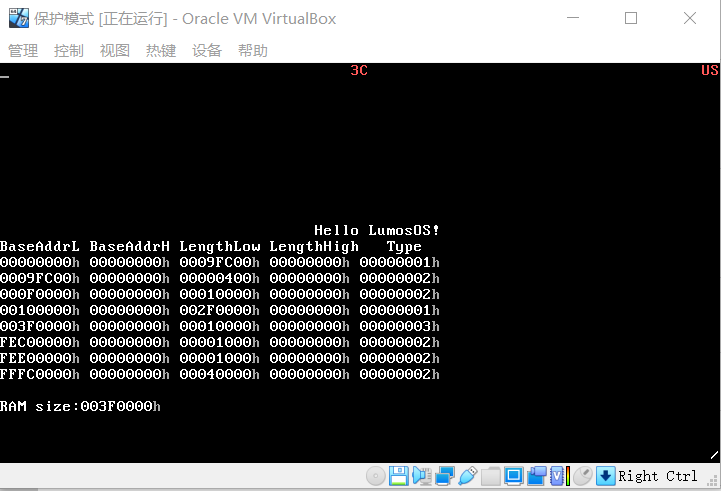
\includegraphics[width=0.7\textwidth]{figs/result.png}
\caption{保护模式LumosOS展示}
\label{fig:result}
\end{figure}

\subsection*{五、实验结果}

\begin{thebibliography}{1}
\bibitem{ref:filesystems} \href{https://blog.csdn.net/goodcrony/article/details/88122934}
{https://blog.csdn.net/goodcrony/article/details/88122934}
一个操作系统的实现
\bibitem{ref:mount} \href{https://www.runoob.com/linux/linux-comm-mount.html}
{https://www.runoob.com/linux/linux-comm-mount.html}
Linux mount命令详解
\bibitem{ref:fat_12} \href{https://zhuanlan.zhihu.com/p/121807427}
{https://zhuanlan.zhihu.com/p/121807427}
FAT12文件系统介绍
\end{thebibliography}

\end{document}